% !TEX root = tesis.tex

\chapter{Clasificación de partículas cargadas y no cargadas en el SciCRT usando un método de anti-coincidencia}
\label{chap:apen-a}

Como mencioné en el capitulo \ref{chap:cuatro}, la separación de las diferentes especies que detecta el SciCRT es una tarea compleja, ya que aunque las capas de muones eliminan la contaminación de partículas cargadas que inciden verticalmente; existe contaminación de partículas cargadas que entran por los lados del detector.

Un método sencillo para eliminar esta contaminación consiste en utilizar las barras que rodean el SB como anti-coincidencia, las cuales se muestran en el figura \ref{fig:scibar-anti} en color verde. Este método funciona debido a que las partículas no cargadas producen trazas en el interior del SB sin disparar la anti coincidencia (traza color rojo en la figura).

\begin{figure}
        \centering
        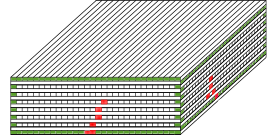
\includegraphics[width=0.6\textwidth]{scibar-anti.pdf}
        \caption{Definición de la señal de anti-coincidencia para el SB3. Las barras color verdes son las utilizadas en el estudio de la eficiencia de separación.}
        \label{fig:scibar-anti}
\end{figure}

Sin embargo este método no es del todo confiable debido a dos problemáticas:

\begin{itemize}
  \item Las barras del SB3 están instaladas a la mitad del detector.
  \item Las barras que se utilizan en anti-coincidencia no están en la capa más exterior del detector (hay \num{16} barras de centelleo extras en cada lado del detector.)
\end{itemize}

El primer punto limita el uso de la capa superior como anti-coincidencia, ya que partículas no cargadas que generen señal en el superior (SB2) podrían ser eliminadas por el uso de el método. El segundo punto disminuye la efectividad del método ya que al cruzar las barras externas al SB, la probabilidad de que neutrones y rayos $\gamma$ interaccionen en las barras de anti-coincidencia.

Considerando esto realicé una simulación MC para encontrar la mejor combinación de patron de anti-coincidencia y umbral para separar partículas cargadas y no cargadas. El resultado de esta simulación se muestra en la figura \ref{fig:anti-patterns}. El panel superior muestra el histograma de deposición de energía de cada de una de las especies en la capa superior del SB3. El panel inferior muestra la misma distribución pero para las barras laterales. De ambas figuras se puede apreciar claramente que todas las especies depositan energía en las barras de anti-coincidencia, por lo que en principio no es posible hacer una separación perfecta.

\begin{figure}
        \centering
        \includegraphics[width=\textwidth]{anti-pattern.pdf}
        \caption{Histogramas de energía depositada para diferentes especies de partículas en la capas de anti-coincidencia.}
        \label{fig:anti-patterns}
\end{figure}

Por esta razón, el patron de anti-coincidencia a usarse en el análisis de los datos debe adecuarse al evento en particular que se esté estudiando. Tomando esto en consideración hay dos casos. Utilizando un umbral de \SI{6.0}{\mega\electronvolt} para las capas de anti-coincidencia, y usando solo las barras de arriba en el disparo: los protones son rechazados en un \SI{90}{\percent}, mientras que neutrones disminuyen en un \SI{50}{\percent} y los muones son prácticamente eliminados.

Con el mismo umbral, pero usando las barras laterales tenemos lo siguiente: protones se eliminan en un \SI{35}{\percent}, mientras que neutrones y muones se atenúan en un \SI{10}{\percent}.

En ambos casos electrones, positrones y rayos $\gamma$ son fuertemente atenuados, por lo que si se desea ver estos productos no se recomienda el uso de la anti-coincidencia.
